\section{\textit{Backend} \textit{Django}}

Para gerenciar, processar e despachar dados, era esperado o desenvolvimento de
um servidor que conseguisse suportar as requisições,
de maneira que não fosse um gargalo para o projeto. Esse requisito foi atingido,
através de um servidor \textit{backend} Django, que hospeda a API que é
utilizada em grande escala pelos clientes (aplicativo Android e servidor
       Ember.JS) e pelo gerador de dados (\textit{middleware}).

Além dos requisitos que estabelecemos nos relatórios anteriores, também
decidimos hospedar o servidor em um ambiente de produção, similar a um cenário
real e profissional. Para o nosso servidor de produção também definimos um
domínio, disponível em \footnote{\url{www.wheelshare-umiss.com/api}}. Por fim,
definimos que por estarmos lidando com dados sigilosos (saúde), adicionamos ao
escopo a adição do HTTPS, que implementamos utilizando os certificados gerados
pelo \textit{let's encrypt}\footnote{\url{https://letsencrypt.org/}}.

Para a documentação da API do projeto, foi utilizada a biblioteca \textit{Swagger},
onde todos os pontos de entrada do software são listadas, bem como os
métodos HTTP possíveis na requisição. A Figura \ref{img:swagger} apresenta
esta funcionalidade.

\begin{figure}
    \begin{center}
        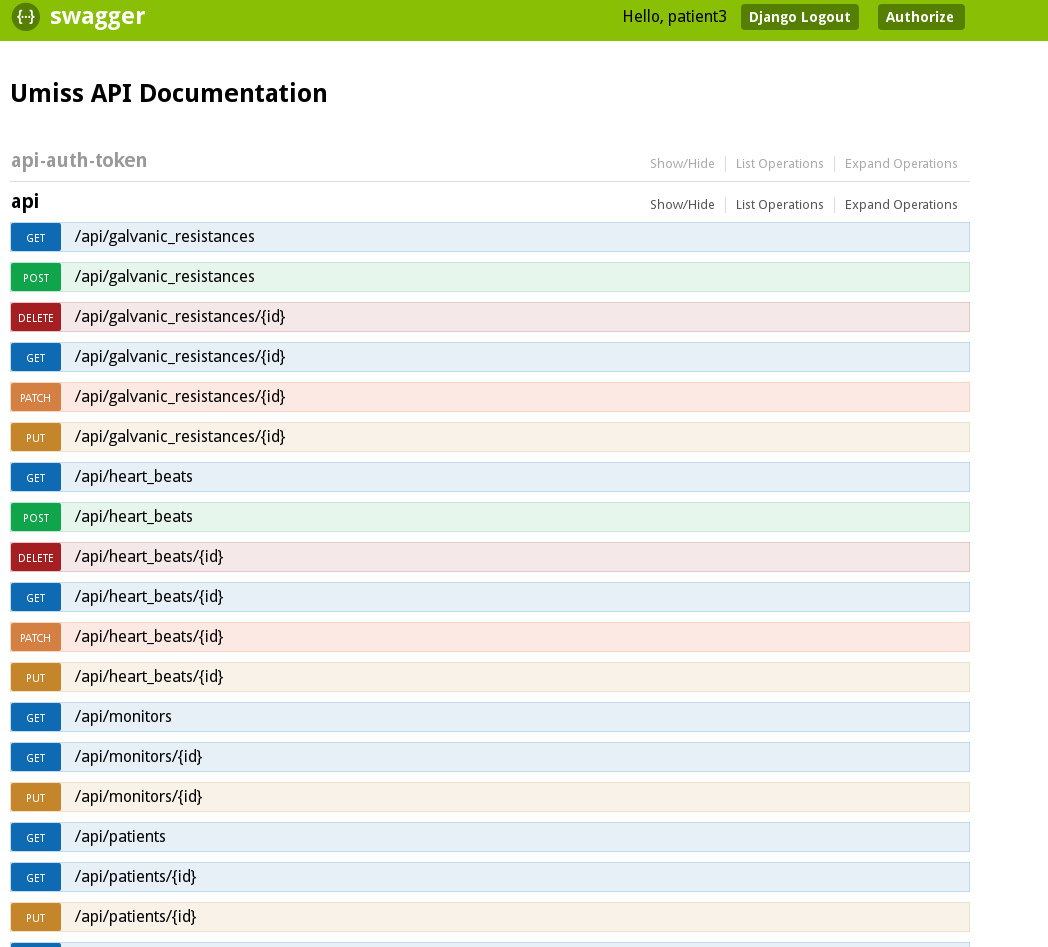
\includegraphics[scale=0.4]{figuras/swagger.png}
    \end{center}
    \caption{Documentação utilizando \textit{Swagger}}
    \label{img:swagger}
\end{figure}
